\section{Vorbereitung}
\label{sec:vorbereitung}


\subsection{Energiestruktur des Atoms}

\subsubsection{Welche Quantenzahlen definieren den Zuestand des Elektrons im Wasserstoffatom?}
$\ket{n,l,m}$
\begin{itemize}
    \item n: Haupt-QZ
    \item l: Bahndrehimpuls QZ
    \item m: magnetische QZ
\end{itemize}

\subsubsection{Was ist die Feinstruktur (Spin-Bahn-Kopplung)?}
\begin{itemize}
    \item WW zwischen Bahndrehimpuls $L$ und Spin $S$
    \item Halbklassisch: 
        \to im Bezugssys. des Elektrons stellt der Kern einen Kreistrom um das Elektron dar
        \to Kreisströme verursachen magnetisches Feld (Biot-Savart) (Kreisstrom entspricht dem Bahndrehimpuls)
        \to dieses magnetische Feld wechselwirkt mit dem magnetischen Moment des Elektronen-Spins
        \to klassisches Analogon: Stabmagnet in Spule
    \item in nicht-relativistischer QM wird ein Störterm $H_S\propto\vec{L}\cdot\vec{S}$ ergänzt
    \item in relativistischer QM ergibt sich die WW automatisch aus der Dirac-Gleichung
\end{itemize}

\subsubsection{Beschreiben Sie die Elektronenkonfiguration und Drehimpulskopplungen in Mehrelektronenatomen (LS-Kopplung und jj-Kopplung)}
\begin{itemize}
    \item Stärke der Spin-Bahn-WW nimmt mit steigendem $Z$ stark zu
    \item Stärke der Spin-Bahn-WW nimmt mit steigendem $n$ ab
\end{itemize}
jj-Kopplung:
\begin{itemize}
    \item Gesamtdrehimpuls aller einzelnen Teilchen werden addiert
    \begin{equation*}
        J=\sum_i j_i=\sum_i(l_i+s_i)\\
    \end{equation*}
    \item elektrostatische Störung der Elektronen untereinander vernachlässigt
    \to Spin-Bahn-WW jedes einzelnen Elektrons >> elektrostatische Störung der Elektronen untereinander
    \iff gute Näherung für mittelschwere Atome auf inneren Schalen und schwere Atome auf ganzen Hülle
\end{itemize}
LS-Kopplung: 
\begin{itemize}
    \item Bahndrehimpuls aller Teilchen und Spin aller Teilchen werden addiert
        \begin{equation*}
            J=L+S=\sum_il_i + \sum_i s_i
        \end{equation*}
    \item Spin-Bahn-WW wird vernachlässigt \iff L und S sind gute QZ 
    \to elektrostatische Störung der Elektronen untereinander >> Spin-Bahn-WW jedes einzelnen Elektrons
    \to gute Näherung für leichte Atome
\end{itemize}


\subsection{Magnetisches Moment des Atoms}

\subsubsection{Wie ist der Zusammenhang zwischen dem magnetischen Moment eines Elektrons und seinen Drehimpulsquantenzahlen?}
\begin{align*}
    \vec{\mu_L}&=-\frac{g_L\mu_B}{\hbar}\vec{L}=-g_L\mu_B\sqrt{l(l+1)}, \quad g_L\approx 1\\
    \vec{\mu_S}&=-\frac{g_S\mu_B}{\hbar}\vec{S}=-g_S\mu_B\sqrt{s(s+1)}, \quad g_S\approx 2
\end{align*}
\subsubsection{Was ist der Unterschied zwischen dem gyromagnetischen Verhältnis für den Elektronenspin und demjenigen für den Drehimpuls?}
\begin{align*}
    \gamma=\frac{|\vec{\mu_l}|}{|\vec{l}|} \qquad
    \gamma=\frac{|\vec{\mu_s}|}{|\vec{s}|}
\end{align*}


\subsection{Aufspaltung des Energieniveaus eines Atoms im homogenen Magnetfeld}

\subsubsection{In wie viele Niveaus spaltet sich der Zustand mit Gesamtdrehimpuls J?}
Durch Spin-Bahn WW: 2 Niveaus\\\noindent
Durch B-Feld: 2 Niveaus

\subsubsection{Wie ändert sich die Aufspaltung mit der Magnetfeldstärke?}
\begin{equation*}
    \Delta E=g_S\mu B_0
\end{equation*}

\subsubsection{Was versteht man unter dem Paschen-Back-Effekt?}
Magnetfeld mit Berücksichtigung des Spins (B>LS-Kopplung)
\to betrachte H-Atom im B-Feld mit LS-Kopplung als Störung


\subsection{Optische Übergänge zwischen Zeemannaufgespaltenen Energieniveaus}
\begin{figure}[H]
    \centering
    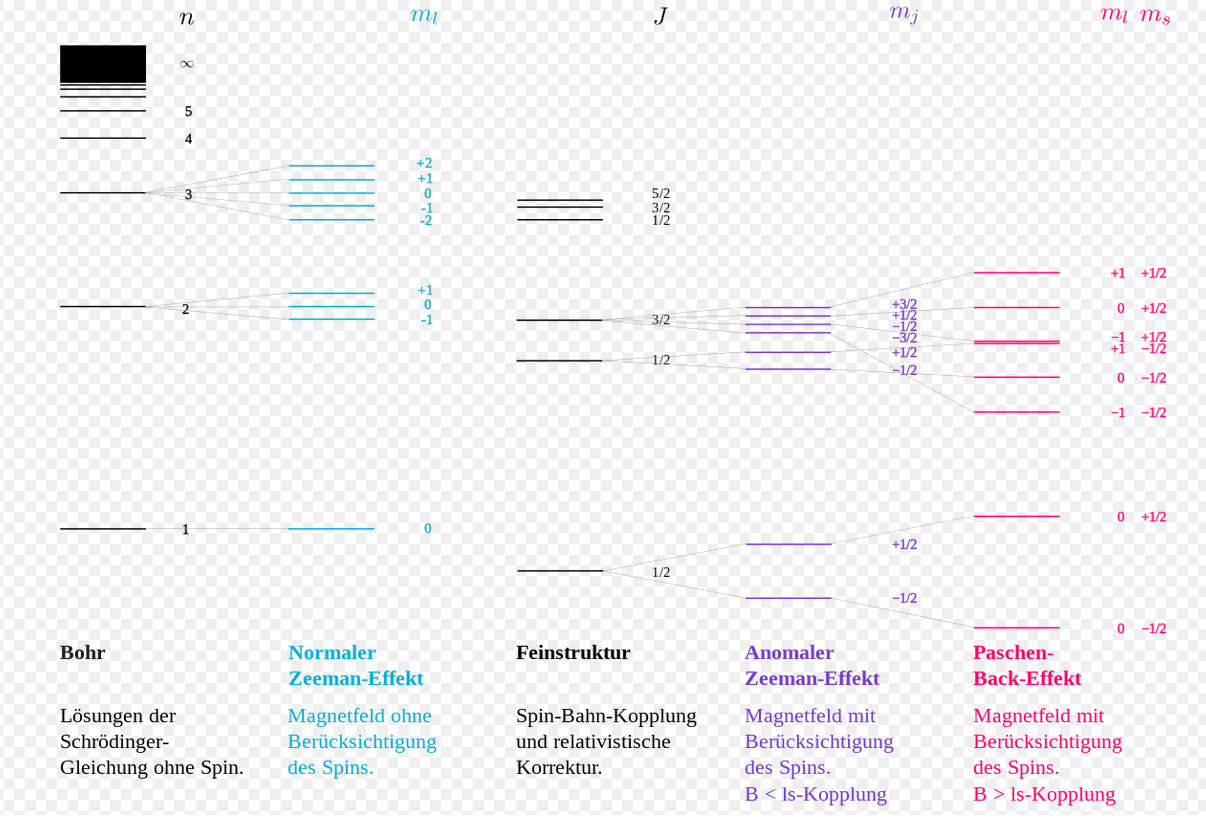
\includegraphics[scale=0.4]{pictures/Aufspaltung.png}
\end{figure}

\subsubsection{Zwischen welchen Zuständen sind optische Übergänge erlaubt?}
Auswahlregeln: 
\begin{align*}
    \Delta l\in\{-1,+1\},\quad\Delta m\in\{-1,0,+1\}
\end{align*}
$\Delta m=0$: $\pi$-Linie
$\Delta m=\pm1$: $\sigma$-Linie

\subsubsection{Wie viele Spektrallinien beobachtet man im normalen und anormalen Zeeman-Effekt?}
normaler Zeeman:  Aufspaltung in $m_L$ \to $2l+1$-Linien
anormaler Zeeman: Aufspaltung in $m_J$ \to $2j+1$-Linien

\subsubsection{Wie sind die Spektrallinien polarisiert?}
\textit{Beachten Sie die geometrischen Verhältnisse des Experiments, d.h. wie ändert sich das Spektrum und die Polarisation der Linien
bei der Beobachtung entlang der Magnetfeldrichtung (longitudinale Geometrie) oder senkrecht zur Magnetfeldrichtung (transversale
Geometrie)?}

\begin{figure}[H] %https://tu-dresden.de/mn/physik/ressourcen/dateien/studium/lehrveranstaltungen/praktika/pdf/ZE.pdf?lang=en
    \centering
    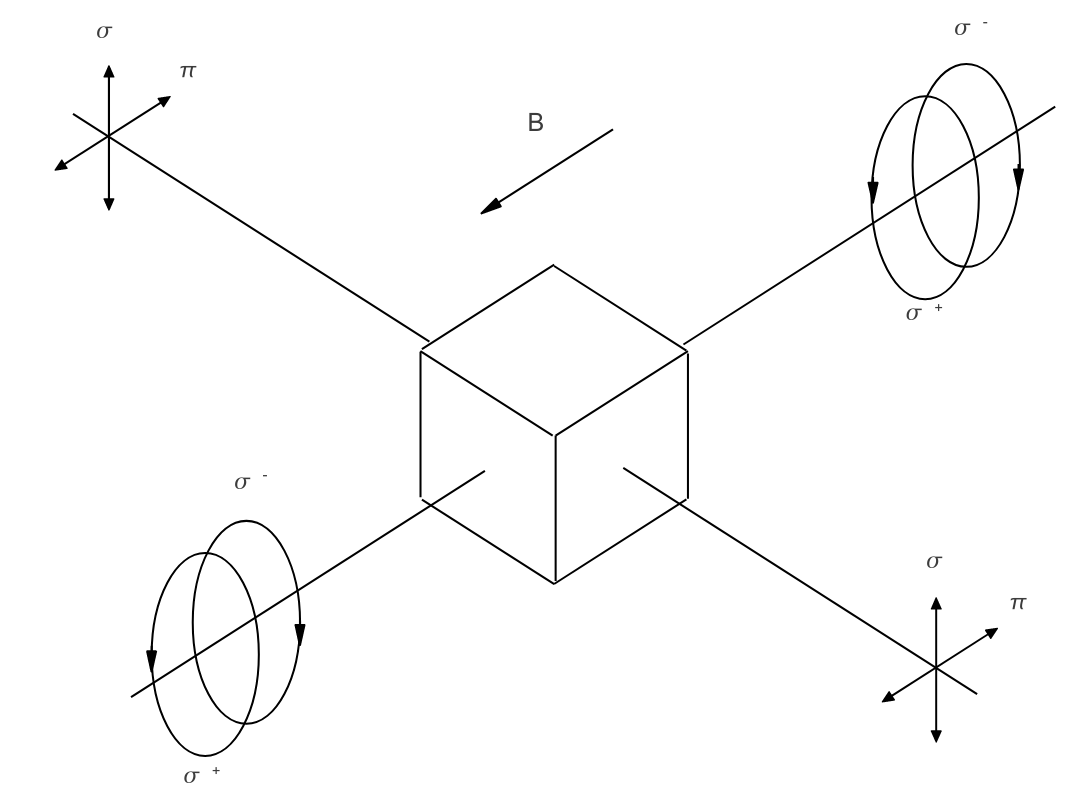
\includegraphics[scale=0.4]{pictures/Polarisation.png}
\end{figure}


\subsection{Optische Übergänge in Cd Atomen}

\subsubsection[]{Stellen Sie das Termschema für die rote $(^1P_1 \leftrightarrow ^1D_2)$ und blaue 
$(^3S_1 \leftrightarrow ^3P_1)$ Linie der Cd-Lampe auf.}
\begin{align*}
    \text{rot: } \quad&^1P_1 \leftrightarrow ^1D_2 \\\iff &S=0, L=0, J=1\leftrightarrow S=0, L=2, J=2 \to\text{normal}\\
    \text{blau:} \quad&^3S_1 \leftrightarrow ^3P_1 \\\iff &S=1, L=0, J=1\leftrightarrow S=1, L=1, J=1 \to\text{anormal}   
\end{align*}

\subsubsection[]{Berechnen Sie die Landé-Faktoren $g_i$ und die Aufspaltung $\Delta E$ der Zeeman-Linie.}
Allgemein:
\begin{equation*}
    g_j=1+\frac{j(j+1)-l(l+1)+s(s+1)}{2j(j+1)}
\end{equation*}
für rot:
\begin{align*}
    g_j(^1P_1)&=1+\frac{1(1+1)-1(1+1)}{2\cdot 1(1+1)}=1\\
    g_j(^3S_1)&=1+\frac{1(1+1)+1(1+1)}{2\cdot 1(1+1)}=2\\
\end{align*}
für blau:
\begin{align*}
    g_j(^1D_2)&=1+\frac{2(2+1)-2(2+1)}{2\cdot 2(2+1)}        &=1\\
    g_j(^3P_1)&=1+\frac{1(1+1)+1(1+1)-1(1+1)}{2\cdot 1(1+1)} &=\frac{3}{2}
\end{align*}

\subsubsection{Zeichnen Sie die erwarteten Spektren.}
\begin{figure}[H] 
    \centering
    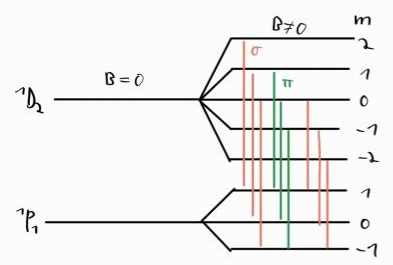
\includegraphics[scale=0.7]{pictures/Aufspaltung_rot.png}
    \caption{Aufspaltung für rot}
\end{figure}
\begin{figure}[H] 
    \centering
    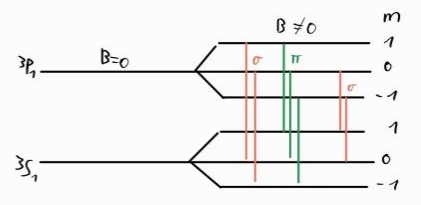
\includegraphics[scale=0.7]{pictures/Aufspaltung_blau.png}
    \caption{Aufspaltung für blau}
\end{figure}

\subsubsection{Wie viele Linien erwarten Sie im Magnetfeld?}
rot: 3 Linien\\\noindent
blau: 3 Linien

\subsubsection{Ordnen Sie den beobachtbaren Linien ihre Polarisation zu.}
$\pi$-Linie: linear\\\noindent
$\sigma$-Linie: zirkular


\subsection{Dispersionsgebiet und spektrale Auflösung der Messapparatur}

\subsubsection[]{Berechnen Sie für $\lambda=\SI{643.8}{\nano\metre}$ und $\lambda=\SI{480}{\nano\metre}$ das Dispersionsgebiet 
$\Delta\lambda_D$  und das Auflösevermögen $A$ der Lummer-Gehrcke-Platte ($d=\SI{4}{\milli\metre}, L=\SI{120}{\milli\metre}, 
n(\SI{643.8}{\nano\metre})=\num{1.4567}, n(\SI{480}{\nano\metre})=\num{1.4635}$).}
Dispersionsgebiet:
\begin{align*}
    \Delta\lambda_D&=\frac{\lambda^2}{2d}\frac{1}{\sqrt{n^2-1}}\\
    \Delta\lambda_D(\SI{643.8}{\nano\metre})&\approx\SI{48.91}{\pico\metre}\\
    \Delta\lambda_D(\SI{480.0}{\nano\metre})&\approx\SI{26.95}{\pico\metre}
\end{align*}
Auflösevermögen:
\begin{align*}
    A&=\frac{L}{\lambda}(n^2-1)\\
    A(\SI{643.8}{\nano\metre})&\approx\num{209128.6}\\
    A(\SI{480.0}{\nano\metre})&\approx\num{285458.1}
\end{align*}


\subsection{Optimale Einstellung der Magnetfeldstärke}

\subsubsection[]{Bestimmen Sie die Bedingung für die optimale Aufspaltung $\Delta\lambda$.}
\textit{Die Messung ist nur sinnvoll für die Aufspaltung innerhalb des Dispersionsgebiets $\Delta\lambda_D$. Das bedeutet, dass 
es eine Begrenzung für die Magnetfeldstärke gibt.}\\
Abstand zwischen den Linien mit und ohne B-Feld:
\begin{align*}
    B=0:    &\Delta s=\Delta\lambda_D\\
    B\neq0: &\delta s=2\delta\lambda_D
\end{align*}
Es gilt
\begin{equation*}
    \delta\lambda=\frac{1}{2}\frac{\delta s}{\Delta s}\Delta\lambda_D=\frac{1}{4}\Delta\lambda_D .
\end{equation*}

\subsubsection{Dauras schätzen Sie die entsprechende optimale Magnetfeldstärke für jede spektrale Linie, die Sie anschließend
messen sollen.}
Energie ist gegeben durch 
\begin{align*}
    E&=\frac{ch}{\lambda}\\
    \Rightarrow \frac{\partial E}{\partial\lambda}&=-\frac{ch}{\lambda^2},
\end{align*}
also ist 
\begin{equation*}
    \Delta E= \frac{-ch}{\lambda^2}\delta\lambda .
\end{equation*}
Demnach ist 
\begin{align*}
    B&=\frac{\Delta E}{\Delta m\mu_B g_j}=\frac{ch}{4\mu_Bg}\frac{\Delta\lambda_D}{\lambda^2}\\
    B(g=1)&\approx\SI{0.63}{\tesla}\\
    B(g=2)&\approx\SI{0.31}{\tesla}\\
    B(g=3/2)&\approx\SI{0.42}{\tesla}\\
    B(g=1/2)&\approx\SI{1.25}{\tesla}
\end{align*}